\documentclass[11pt]{article}

%=================================================
% PACKAGES
%=================================================

\usepackage[a4paper,margin=2cm]{geometry}

\usepackage[utf8]{inputenc}
\usepackage[T1]{fontenc}

\usepackage{booktabs}
\usepackage{tabularx}

%=================================================
% TYPOGRAPHY
%=================================================

% Use the standard LaTeX fonts for maximum portability.  This avoids local
% font-generation dependencies and compiles unchanged on Overleaf.

\usepackage{amsmath}
\usepackage{amssymb}

% Minimal Dirac-notation helpers.  Keeping these definitions local avoids
% requiring the large physics package on a fresh Overleaf/MiKTeX setup.
\newcommand{\ket}[1]{\left|#1\right\rangle}
\newcommand{\bra}[1]{\left\langle#1\right|}
\newcommand{\mel}[3]{\left\langle#1\right|#2\left|#3\right\rangle}
\newcommand{\matrixel}[3]{\left\langle#1\right|#2\left|#3\right\rangle}
\newcommand{\Tr}{\operatorname{Tr}}
\newcommand{\dv}[2]{\frac{\mathrm{d}#1}{\mathrm{d}#2}}

%=================================================
% EQUATION NUMBERING
%=================================================

\numberwithin{equation}{section}

%=================================================
% FIGURES
%=================================================

\usepackage{graphicx}
\usepackage{xcolor}

\usepackage{hyperref}
\usepackage{xurl}

\usepackage{enumitem}
\usepackage{titlesec}
\usepackage{tcolorbox}
\usepackage{fancyhdr}

\usepackage[numbers,sort&compress]{natbib}

%=================================================
% COLORS
%=================================================

\definecolor{mainblue}{RGB}{0,70,140}

%=================================================
% HYPERLINKS
%=================================================

\hypersetup{
colorlinks=true,
linkcolor=mainblue,
urlcolor=blue,
citecolor=mainblue
}

%=================================================
% HEADINGS
%=================================================
\usepackage{titlesec}

\titleformat{\section}
{\Large\bfseries\color{mainblue}}
{\thesection}
{1em}
{}

% \titleformat{\section}
% {\Large\bfseries\color{mainblue}}
% {\thesection.}{0.5em}{}

\titleformat{\subsection}
{\large\bfseries}
{\thesubsection.}{0.5em}{}

%=================================================
% TABLE OF CONTENTS DEPTH
%=================================================

\setcounter{secnumdepth}{3}
\setcounter{tocdepth}{3}

%=================================================
% BOXES
%=================================================

\newtcolorbox{idea}{
colback=blue!5,
colframe=mainblue,
title=Key idea
}

%=================================================
% HEADER
%=================================================

\pagestyle{fancy}
\setlength{\headheight}{14pt}
\setlength{\emergencystretch}{2em}

\fancyhf{}

\fancyhead[L]{\itshape Technical Progress Report}
\fancyhead[R]{\itshape QuAntü Project}

\fancyfoot[L]{Alexis R. Legón}
\fancyfoot[C]{\thepage}
\fancyfoot[R]{2026}

%=================================================
% DOCUMENT
%=================================================

\begin{document}

%=================================================
% TITLE PAGE
%=================================================

% \noindent
% \textit{Open Quantum Systems}
% \hfill
% \textit{Scientific exploration guide}

\vspace{0.3cm}

\begin{center}

{\Huge\bfseries\color{mainblue}
Technical Progress Report
}

\vspace{0.4cm}

{\LARGE\bfseries
Development of Progressive Theoretical Models\\
for the Rubidium Absorption Spectrum
}

\vspace{0.3cm}

{\large\itshape
Project QuAntü
}

\vspace{0.45cm}

\hrule

\vspace{0.45cm}

{\Large\bfseries Alexis R. Legón}

\vspace{0.15cm}

Pontificia Universidad Católica de Chile\\
QuAntü Research Group

\vspace{0.15cm}

\texttt{alexis.legon@uc.cl}

\vspace{0.4cm}

Reporting Period\\
{\large May 2026 -- July 2026}

\vspace{0.45cm}

\hrule

\end{center}

\vspace{0.02cm}

%=================================================
% TABLE OF CONTENTS
%=================================================

\clearpage
\tableofcontents

\newpage

%%%%%%%%%%%%%%%%%%%%%%%%%%%%%%%%%%%%%%%%%%%%%%%%%%%%%%%%%%%%%%%%%%%%%%%%%%%%%%%%
\section{Executive Summary}
%%%%%%%%%%%%%%%%%%%%%%%%%%%%%%%%%%%%%%%%%%%%%%%%%%%%%%%%%%%%%%%%%%%%%%%%%%%%%%%%

This report summarizes the research activities carried out during the present reporting period within the QuAntü research project at the Pontificia Universidad Católica de Chile. The work focuses on the theoretical modeling of the absorption spectrum of natural-abundance rubidium vapor, with the objective of developing progressively more realistic microscopic descriptions of light--matter interactions in atomic systems.

During this period, a systematic theoretical framework was established by progressively incorporating the dominant physical mechanisms governing the observed absorption spectrum. The research began with a phenomenological Gaussian description of Doppler broadening, followed by the explicit inclusion of the natural isotopic composition of rubidium and a microscopic optical-susceptibility model. The framework was then extended to a full steady-state density-matrix calculation that resolves every D2 hyperfine and magnetic sublevel of both abundant isotopes. The earlier stages were validated against reconstructed experimental spectra, while the density-matrix implementation was verified against atomic constants, transition centers, selection rules, and an independent direct-solver formulation.

In parallel with the development of the theoretical models, an extensive literature review was conducted covering experimental spectroscopy, susceptibility-based approaches, rate-equation models, density-matrix formulations, and the detailed rubidium data compilations of Steck. This analysis supplied the hyperfine constants, isotope shift, wavelengths, natural linewidths, angular-momentum reduction formulas, and optical-pumping theory used in the implementation.

The results establish a computational and theoretical platform that connects phenomenological spectra to open-system atomic dynamics. The new master-equation model includes coherent laser coupling, spontaneous-emission branching, phenomenological ground-state remixing, optical pumping, saturation, Doppler averaging, and natural-isotope mixing. The remaining step toward parameter-free quantitative spectroscopy is to replace the empirical frequency and optical-depth calibrations by independently measured experimental parameters.

%%%%%%%%%%%%%%%%%%%%%%%%%%%%%%%%%%%%%%%%%%%%%%%%%%%%%%%%%%%%%%%%%%%%%%%%%%%%%%%%
\section{Project Objectives}
%%%%%%%%%%%%%%%%%%%%%%%%%%%%%%%%%%%%%%%%%%%%%%%%%%%%%%%%%%%%%%%%%%%%%%%%%%%%%%%%

The primary objective of this project is to develop a progressively more realistic theoretical framework for describing the optical absorption spectrum of thermal rubidium vapor. Starting from simple phenomenological models and advancing toward microscopic quantum descriptions, the project aims to identify the physical mechanisms governing the observed spectral features while establishing a computational platform for quantitative spectroscopy.

During the present reporting period, the research focused on the implementation and validation of successive theoretical models with increasing levels of physical complexity. The work began with a phenomenological Gaussian description of Doppler broadening, followed by the natural-isotope and microscopic optical-susceptibility models, and culminated in a Zeeman-resolved density-matrix solver for the D2 manifolds of \(^{85}\mathrm{Rb}\) and \(^{87}\mathrm{Rb}\).

Beyond reproducing experimental spectra, the project seeks to establish a unified and reproducible modeling framework. The implemented optical Bloch and density-matrix approach now provides the basis for investigating nonlinear optical phenomena, optical pumping, coherent light--matter interactions, and open quantum dynamics relevant to quantum technologies.

%%%%%%%%%%%%%%%%%%%%%%%%%%%%%%%%%%%%%%%%%%%%%%%%%%%%%%%%%%%%%%%%%%%%%%%%%%%%%%%%
\section{Activities Performed}
%%%%%%%%%%%%%%%%%%%%%%%%%%%%%%%%%%%%%%%%%%%%%%%%%%%%%%%%%%%%%%%%%%%%%%%%%%%%%%%%

During the present reporting period, the research activities focused on the development and validation of theoretical models for describing the optical absorption spectrum of thermal rubidium vapor. The work followed a progressive modeling strategy, beginning with simple phenomenological descriptions and systematically incorporating additional physical mechanisms to achieve increasingly accurate agreement with experimental observations.

The activities carried out can be grouped into the following stages:

\begin{enumerate}
    \item Literature review and theoretical background.
    \item Analysis of the experimental absorption spectrum.
    \item Development of progressively more realistic theoretical models.
    \item Numerical implementation and validation of each model.
    \item Comparison with experimental data and assessment of model performance.
\end{enumerate}

%%%%%%%%%%%%%%%%%%%%%%%%%%%%%%%%%%%%%%%%%%%%%%%%%%%%%%%%%%%%%%%%%%%%%%%%%%%%%%%%
\subsection{Literature Review}
%%%%%%%%%%%%%%%%%%%%%%%%%%%%%%%%%%%%%%%%%%%%%%%%%%%%%%%%%%%%%%%%%%%%%%%%%%%%%%%%

The first stage of this project consisted of a comprehensive literature review to establish the theoretical and experimental foundations for modeling the optical absorption spectrum of thermal rubidium vapor. The objective was to identify the physical mechanisms governing the observed spectral features and to define a systematic strategy for the progressive development of increasingly realistic theoretical models.

The review covered experimental absorption measurements \cite{Ma2017}, spectroscopic techniques including Doppler-free spectroscopy \cite{Jacques2009}, susceptibility-based models \cite{Siddons2008,Agnew2024}, rate-equation approaches \cite{Bala2022}, and density-matrix methods based on the optical Bloch equations \cite{Horn2011}. Together, these studies provided the theoretical framework adopted throughout this project.

Based on this review, a progressive modeling methodology was established, where each successive model incorporates additional physical mechanisms while preserving the physical insight gained from the previous description. This strategy forms the basis for the theoretical developments presented in the following sections.

%%%%%%%%%%%%%%%%%%%%%%%%%%%%%%%%%%%%%%%%%%%%%%%%%%%%%%%%%%%%%%%%%%%%%%%%%%%%%%%%
\subsection{Experimental Dataset}
%%%%%%%%%%%%%%%%%%%%%%%%%%%%%%%%%%%%%%%%%%%%%%%%%%%%%%%%%%%%%%%%%%%%%%%%%%%%%%%%

To validate the theoretical models developed in this project, a reference experimental dataset was reconstructed from the published absorption spectrum reported by Ma \textit{et al.} \cite{Ma2017}. The selected spectrum corresponds to thermal rubidium vapor with natural isotopic abundance and provides a high-quality benchmark for comparison with theoretical calculations.

The published absorption spectrum was digitally extracted and normalized to generate a numerical dataset suitable for quantitative analysis. This reconstructed dataset was subsequently used as the common reference for evaluating the successive theoretical models developed throughout this project. By comparing the calculated spectra with the experimental measurements, it was possible to assess the accuracy of each model and identify the physical mechanisms required for a progressively more realistic description of the rubidium absorption spectrum.

%%%%%%%%%%%%%%%%%%%%%%%%%%%%%%%%%%%%%%%%%%%%%%%%%%%%%%%%%%%%%%%%%%%%%%%%%%%%%%%%
\subsection{Progressive Development of Theoretical Models}
%%%%%%%%%%%%%%%%%%%%%%%%%%%%%%%%%%%%%%%%%%%%%%%%%%%%%%%%%%%%%%%%%%%%%%%%%%%%%%%%

%%%%%%%%%%%%%%%%%%%%%%%%%%%%%%%%%%%%%%%%%%%%%%%%%%%%%%%%%%%%%%%%%%%%%%%%%%%%%%%%
\subsubsection{Phenomenological Gaussian Model}
%%%%%%%%%%%%%%%%%%%%%%%%%%%%%%%%%%%%%%%%%%%%%%%%%%%%%%%%%%%%%%%%%%%%%%%%%%%%%%%%

As a first approximation, the absorption spectrum of thermal rubidium vapor was described using a phenomenological Gaussian model that accounts only for Doppler broadening. At room temperature, Doppler broadening is the dominant mechanism determining the spectral linewidth, making this simplified description an appropriate starting point for the progressive development of more realistic theoretical models.

Under this approximation, each absorption resonance is represented by an effective Gaussian profile sharing a common Doppler linewidth. The resulting phenomenological absorption model is given by Eq.~(\ref{eq:gaussian_model}),

\begin{equation}
\label{eq:gaussian_model}
A(\Omega)=
\sum_i A_i
\exp\left[
-\frac{(\Omega-\Omega_i)^2}{2\sigma^2}
\right],
\end{equation}

where $A_i$ and $\Omega_i$ denote the effective amplitude and central frequency of the $i$-th absorption resonance, respectively, while $\sigma$ represents the common Doppler linewidth. In this model, the resonance amplitudes and positions are treated as phenomenological fitting parameters, and the isotopic and hyperfine structures of natural rubidium are not explicitly included.

Figure~\ref{fig:gaussian_model} compares the phenomenological Gaussian model with the reconstructed experimental absorption spectrum. The model successfully reproduces the overall spectral profile and captures the four dominant absorption resonances observed experimentally. However, the resonance positions require phenomenological adjustments, and the model does not provide a microscopic interpretation of the isotopic and hyperfine structure. These limitations motivate the introduction of increasingly realistic theoretical descriptions in the following sections.

\begin{figure}[t]
\centering
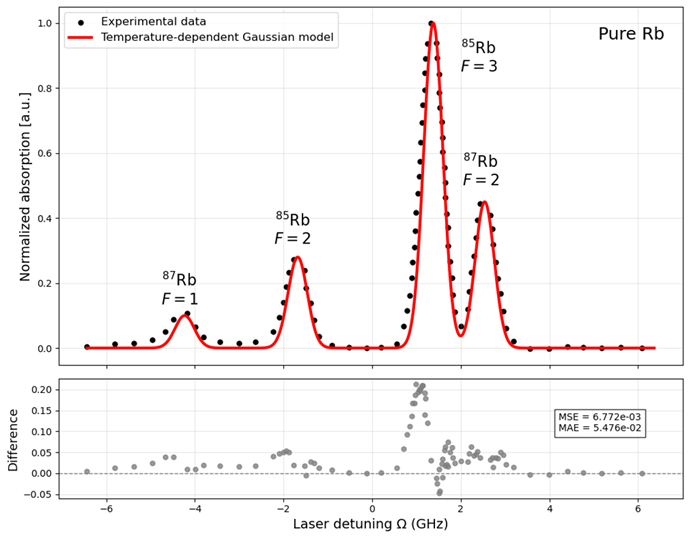
\includegraphics[width=0.75\textwidth]{figure_1.png}
\caption{Comparison between the phenomenological Gaussian model and the reconstructed experimental absorption spectrum. The model reproduces the overall spectral profile and the four dominant absorption resonances but does not explicitly incorporate the isotopic and hyperfine structure of natural rubidium.}
\label{fig:gaussian_model}
\end{figure}


%%%%%%%%%%%%%%%%%%%%%%%%%%%%%%%%%%%%%%%%%%%%%%%%%%%%%%%%%%%%%%%%%%%%%%%%%%%%%%%%
\subsubsection{Gaussian Model with Natural Isotopic Composition}
%%%%%%%%%%%%%%%%%%%%%%%%%%%%%%%%%%%%%%%%%%%%%%%%%%%%%%%%%%%%%%%%%%%%%%%%%%%%%%%%

Building upon the phenomenological Gaussian model, the second approach explicitly incorporates the natural isotopic composition of rubidium. Since naturally occurring rubidium consists of approximately 72.17\% $^{85}$Rb and 27.83\% $^{87}$Rb, the absorption spectrum is modeled as the superposition of the independent contributions from both isotopes while retaining Doppler broadening as the dominant linewidth mechanism.

Under this approximation, the total absorption spectrum is expressed as the sum of the isotopic contributions according to Eq.~(\ref{eq:isotopic_model}),

\begin{equation}
\label{eq:isotopic_model}
A(\Omega)=A_{85}(\Omega)+A_{87}(\Omega),
\end{equation}

where $A_{85}(\Omega)$ and $A_{87}(\Omega)$ denote the effective Doppler-broadened absorption spectra associated with the $^{85}$Rb and $^{87}$Rb isotopes, respectively. Each isotopic contribution is represented by effective Gaussian resonances corresponding to the experimentally observed hyperfine transitions, while the natural isotopic abundances are explicitly incorporated into the model.

Figure~\ref{fig:isotopic_model} compares the calculated spectrum with the reconstructed experimental dataset. Incorporating the natural isotopic composition significantly improves the agreement with the experimental spectrum by providing a physical interpretation of the four dominant absorption resonances. In particular, the model yields more accurate resonance positions and relative peak amplitudes while preserving the simplicity of the phenomenological Gaussian description. These results demonstrate that explicitly accounting for the isotopic composition constitutes an important step toward a more realistic description of the rubidium absorption spectrum.

\begin{figure}[t]
\centering
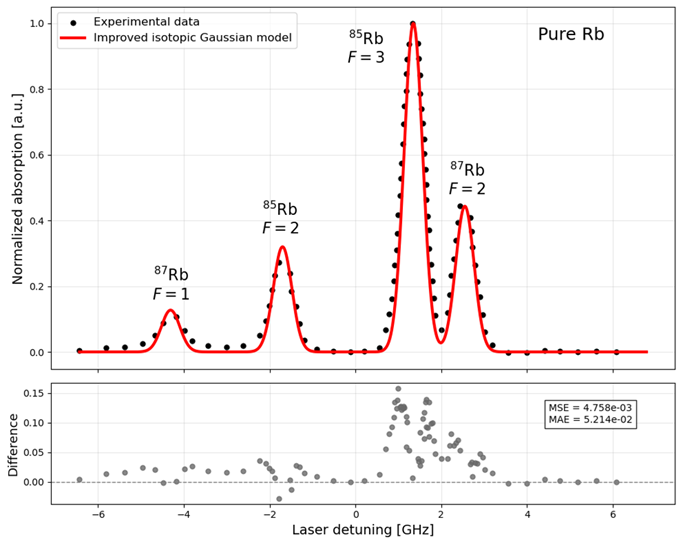
\includegraphics[width=0.75\textwidth]{figure_2.png}
\caption{Comparison between the Gaussian model including the natural isotopic composition of rubidium and the reconstructed experimental absorption spectrum. Explicitly incorporating the contributions of the $^{85}$Rb and $^{87}$Rb isotopes improves the agreement with the experimental data and provides a physical interpretation of the observed absorption resonances.}
\label{fig:isotopic_model}
\end{figure}


%%%%%%%%%%%%%%%%%%%%%%%%%%%%%%%%%%%%%%%%%%%%%%%%%%%%%%%%%%%%%%%%%%%%%%%%%%%%%%%%
\subsubsection{Microscopic Optical Susceptibility Model}
%%%%%%%%%%%%%%%%%%%%%%%%%%%%%%%%%%%%%%%%%%%%%%%%%%%%%%%%%%%%%%%%%%%%%%%%%%%%%%%%

The third model adopts a microscopic description of the rubidium absorption spectrum based on the optical susceptibility of the atomic medium. Unlike the previous phenomenological approaches, the absorption spectrum is directly obtained from the optical response of the atomic vapor, providing a physically grounded description of the light--matter interaction.

Within the weak-probe approximation, the optical susceptibility is described by Eq.~(\ref{eq:susceptibility}),

\begin{equation}
\label{eq:susceptibility}
\chi(\omega)=
\sum_i
\frac{A_i}
{\omega-\omega_i+i\Gamma_i},
\end{equation}

where $A_i$, $\omega_i$, and $\Gamma_i$ denote the transition strength, resonance frequency, and homogeneous linewidth of the $i$-th transition, respectively. The absorption spectrum is proportional to the imaginary part of the optical susceptibility and incorporates Doppler broadening by averaging over the Maxwell--Boltzmann velocity distribution according to Eq.~(\ref{eq:doppler_average}),

\begin{equation}
\label{eq:doppler_average}
\chi_D(\omega)=
\int dv\,f(v)\,\chi(\omega,v),
\end{equation}

where $f(v)$ is the Maxwell--Boltzmann velocity distribution.

Figure~\ref{fig:susceptibility_model} compares the microscopic susceptibility model with the reconstructed experimental absorption spectrum. The inclusion of both homogeneous and Doppler broadening yields the best agreement with the experimental data among the models considered in this work. Furthermore, the model provides a microscopic description of the optical response and achieves the lowest mean squared error (MSE) and mean absolute error (MAE), demonstrating its superior accuracy for describing the absorption spectrum of thermal rubidium vapor.

\begin{figure}[t]
\centering
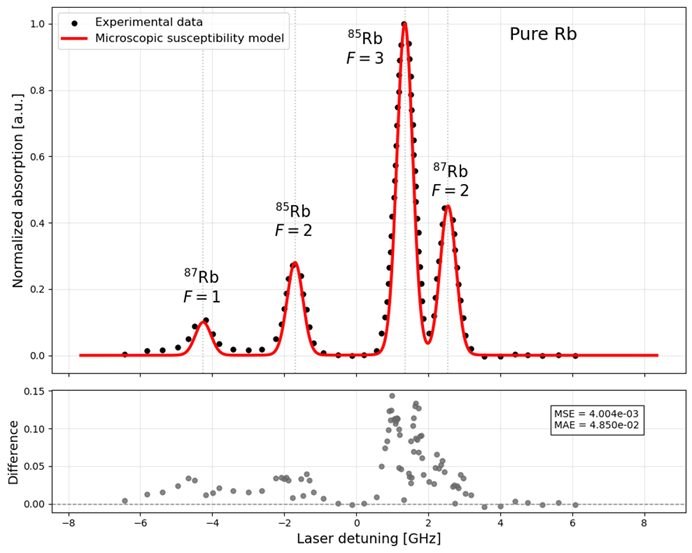
\includegraphics[width=0.75\textwidth]{figure_3.png}
\caption{Comparison between the microscopic optical susceptibility model and the reconstructed experimental absorption spectrum. The susceptibility-based model incorporates both homogeneous and Doppler broadening, providing the best agreement with the experimental data and the most accurate microscopic description of the optical response.}
\label{fig:susceptibility_model}
\end{figure}

%%%%%%%%%%%%%%%%%%%%%%%%%%%%%%%%%%%%%%%%%%%%%%%%%%%%%%%%%%%%%%%%%%%%%%%%%%%%%%%%
% FULL DENSITY-MATRIX MODEL
%%%%%%%%%%%%%%%%%%%%%%%%%%%%%%%%%%%%%%%%%%%%%%%%%%%%%%%%%%%%%%%%%%%%%%%%%%%%%%%%

\clearpage
%%%%%%%%%%%%%%%%%%%%%%%%%%%%%%%%%%%%%%%%%%%%%%%%%%%%%%%%%%%%%%%%%%%%%%%%%%%%%%%%
\section[Full Density-Matrix Model for the Rubidium D2 Absorption Spectrum]
{Full Density-Matrix Model for the\\Rubidium D2 Absorption Spectrum}
\label{sec:density_matrix_model}
%%%%%%%%%%%%%%%%%%%%%%%%%%%%%%%%%%%%%%%%%%%%%%%%%%%%%%%%%%%%%%%%%%%%%%%%%%%%%%%%

This section derives, from first principles, the model implemented in the
MATLAB script
\begin{center}
\path{Rb_D2_density_matrix_fast_COHERENCE_ABS.m}.
\end{center}
The purpose is not only to state the equations, but also to explain how every
physical object becomes a MATLAB array and how the final absorption curve is
constructed.  The
derivation follows the angular-momentum and spectroscopic conventions tabulated
by Steck for \(^{85}\mathrm{Rb}\) and \(^{87}\mathrm{Rb}\)
\cite{Steck85,Steck87}.

\begin{idea}
The calculation has four layers.  First, atomic angular momentum determines
the hyperfine--Zeeman basis and its energies.  Second, the laser polarization
and the Wigner--Eckart theorem determine which states are coupled and with what
relative amplitude.  Third, a Lindblad master equation determines the
steady-state populations and coherences.  Finally, the absorptive optical
coherence is averaged over the thermal velocity distribution and converted to
a transmitted-intensity loss.
\end{idea}

%%%%%%%%%%%%%%%%%%%%%%%%%%%%%%%%%%%%%%%%%%%%%%%%%%%%%%%%%%%%%%%%%%%%%%%%%%%%%%%%
\subsection{Physical Scope and Modeling Chain}
\label{subsec:dm_scope}
%%%%%%%%%%%%%%%%%%%%%%%%%%%%%%%%%%%%%%%%%%%%%%%%%%%%%%%%%%%%%%%%%%%%%%%%%%%%%%%%

The experiment probes the rubidium D2 transition,
\begin{equation}
5^{2}S_{1/2}\longrightarrow 5^{2}P_{3/2},
\end{equation}
near \(780~\mathrm{nm}\).  Natural rubidium contains two abundant isotopes.
The code treats the two isotopes as independent atomic gases, calculates one
spectrum for each isotope, and combines the two spectra using the natural
abundances.  Within each isotope, all hyperfine levels and all magnetic
sublevels \(m_F\) of the D2 line are retained.

The calculation can be summarized as
\begin{equation}
\begin{split}
\{I,J,F,m_F,A,B\}
&\longrightarrow
\{\ket{g;F,m_F},\ket{e;F',m_F'}\}
\\
&\longrightarrow
H_{\mathrm{hfs}}+H_{\mathrm{laser}}
\\
&\longrightarrow
\mathcal{L}(x)\rho_{\mathrm{ss}}(x)=0
\\
&\longrightarrow
\operatorname{Im}\!\left[
\sum_{g,e}d_{eg}^{*}\rho_{ge}^{\mathrm{ss}}(x)
\right]
\\
&\longrightarrow
\text{Doppler average}
\longrightarrow
\text{isotopic mixture}
\longrightarrow
\text{absorption}.
\end{split}
\label{eq:dm_model_chain}
\end{equation}
Here \(x\) is the detuning experienced by one velocity class.  The central
numerical advantage of the ``fast'' implementation is that the steady state is
solved once as a function of \(x\), rather than once for every pair of laser
frequency and atomic velocity.

%%%%%%%%%%%%%%%%%%%%%%%%%%%%%%%%%%%%%%%%%%%%%%%%%%%%%%%%%%%%%%%%%%%%%%%%%%%%%%%%
\subsection{Atomic Structure and Hilbert-Space Basis}
\label{subsec:dm_atomic_basis}
%%%%%%%%%%%%%%%%%%%%%%%%%%%%%%%%%%%%%%%%%%%%%%%%%%%%%%%%%%%%%%%%%%%%%%%%%%%%%%%%

\subsubsection{From electronic to total atomic angular momentum}

For an alkali atom, the single valence electron has orbital angular momentum
\(\mathbf{L}\) and spin \(\mathbf{S}\).  These combine to give
\begin{equation}
\mathbf{J}=\mathbf{L}+\mathbf{S}.
\end{equation}
For the D2 line,
\begin{equation}
J_g=\frac{1}{2}
\qquad\text{and}\qquad
J_e=\frac{3}{2},
\end{equation}
where \(g\) and \(e\) label the ground and excited fine-structure manifolds.
The electronic angular momentum then couples to the nuclear spin
\(\mathbf{I}\):
\begin{equation}
\mathbf{F}=\mathbf{I}+\mathbf{J},
\qquad
F=|I-J|,|I-J|+1,\ldots,I+J.
\label{eq:F_addition}
\end{equation}
Finally, each hyperfine level \(F\) contains \(2F+1\) magnetic sublevels
\begin{equation}
m_F=-F,-F+1,\ldots,F.
\end{equation}

The isotopes have different nuclear spins and therefore different hyperfine
manifolds.  The exact basis used by the code is listed in
Table~\ref{tab:dm_basis}.

\begin{table}[t]
\centering
\small
\renewcommand{\arraystretch}{1.15}
\caption{Hyperfine--Zeeman basis retained for each isotope.}
\label{tab:dm_basis}
\begin{tabular}{ccccc}
\toprule
Isotope & \(I\) & Ground \(F\) & Excited \(F'\) & Dimensions \((N_g,N_e,N)\) \\
\midrule
\(^{85}\mathrm{Rb}\) & \(5/2\) & \(2,3\) & \(1,2,3,4\) & \((12,24,36)\) \\
\(^{87}\mathrm{Rb}\) & \(3/2\) & \(1,2\) & \(0,1,2,3\) & \((8,16,24)\) \\
\bottomrule
\end{tabular}
\end{table}

For example, the \(^{85}\mathrm{Rb}\) ground manifold has
\((2\times2+1)+(2\times3+1)=5+7=12\) states.  Its excited manifold has
\(3+5+7+9=24\) states, so the Hilbert-space dimension is \(N=36\).
A density matrix is an \(N\times N\) matrix; after vectorization, the
corresponding Liouville-space dimensions are therefore
\begin{equation}
N_{85}^{2}=1296,
\qquad
N_{87}^{2}=576.
\end{equation}

The MATLAB function \texttt{build\_basis} creates one structure for every
\(\ket{g;F,m_F}\) and \(\ket{e;F',m_F'}\).  Each structure stores the
manifold label, \(F\), \(m_F\), hyperfine energy in MHz, and a unique matrix
index.  No Zeeman energy is added in the present version.  Thus, the
\(m_F\) states are explicitly present so that polarization selection rules,
optical pumping, and spontaneous-emission branching can be modeled, but they
remain degenerate in the field-free Hamiltonian.

\subsubsection{Hyperfine Hamiltonian and level energies}

The magnetic-dipole and electric-quadrupole hyperfine interactions are
described by \cite{Steck85,Steck87}
\begin{equation}
H_{\mathrm{hfs}}
=
A_{\mathrm{hfs}}\,\mathbf{I}\cdot\mathbf{J}
+
B_{\mathrm{hfs}}
\frac{
3(\mathbf{I}\cdot\mathbf{J})^{2}
+\frac{3}{2}\mathbf{I}\cdot\mathbf{J}
-I(I+1)J(J+1)
}{
2I(2I-1)J(2J-1)
}.
\label{eq:hyperfine_hamiltonian}
\end{equation}
Because the basis states \(\ket{F,m_F}\) are eigenstates of
\(\mathbf{F}^{2}\), one uses
\begin{equation}
\mathbf{I}\cdot\mathbf{J}
=
\frac{1}{2}
\left[
F(F+1)-I(I+1)-J(J+1)
\right].
\end{equation}
Defining
\begin{equation}
K=F(F+1)-I(I+1)-J(J+1),
\label{eq:hyperfine_K}
\end{equation}
the frequency shift of a hyperfine level relative to the fine-structure
center of gravity is
\begin{equation}
\frac{E_{\mathrm{hfs}}(F)}{h}
=
\frac{A_{\mathrm{hfs}}}{2}K
+
B_{\mathrm{hfs}}
\frac{
\frac{3}{2}K(K+1)-2I(I+1)J(J+1)
}{
4I(2I-1)J(2J-1)
}.
\label{eq:hyperfine_shift}
\end{equation}
Equation~\eqref{eq:hyperfine_shift} is implemented directly by
\texttt{hyperfine\_shift\_MHz}.  The constants \(A_{\mathrm{hfs}}\) and
\(B_{\mathrm{hfs}}\) are entered in MHz, so the returned value is
\(E_{\mathrm{hfs}}/h\) in MHz.  The quadrupole term is omitted when
\(J=1/2\), because a \(J=1/2\) state has no electric-quadrupole hyperfine
splitting.

\begin{table}[t]
\centering
\small
\renewcommand{\arraystretch}{1.15}
\caption{Hyperfine constants used by the script.  All values are in MHz.}
\label{tab:dm_hfs_constants}
\begin{tabular}{ccccc}
\toprule
Isotope & \(A_g(5^2S_{1/2})\) & \(B_g\) &
\(A_e(5^2P_{3/2})\) & \(B_e(5^2P_{3/2})\) \\
\midrule
\(^{85}\mathrm{Rb}\) & \(1011.9108130\) & \(0\) &
\(25.0354\) & \(25.898\) \\
\(^{87}\mathrm{Rb}\) & \(3417.341305452145\) & \(0\) &
\(84.7185\) & \(12.4965\) \\
\bottomrule
\end{tabular}
\end{table}

These numbers are taken from the isotope data compilations
\cite{Steck85,Steck87}.  The large difference between the ground-state and
excited-state splittings explains why the four principal Doppler-broadened
groups are associated mainly with the two ground hyperfine levels of each
isotope.

\subsubsection{Frequency origin, isotope shift, and transition centers}

The script uses a detuning convention that is the negative of a common
laser-minus-atom convention:
\begin{equation}
\Omega=\nu_{85,\mathrm{D2\,cog}}-\nu_L,
\label{eq:Omega_convention}
\end{equation}
where ``cog'' denotes the fine-structure center of gravity and all frequencies
in Eq.~\eqref{eq:Omega_convention} are ordinary frequencies, not angular
frequencies.  Therefore increasing the laser frequency moves \(\Omega\) in
the negative direction.

The \(^{85}\mathrm{Rb}\) D2 center is defined as zero.  The
\(^{87}\mathrm{Rb}\) D2 center is higher in optical frequency by
\begin{equation}
\delta_{\mathrm{iso}}^{87-85}=78.095~\mathrm{MHz}
\label{eq:isotope_shift}
\end{equation}
\cite{Steck85}.  For a stationary atom, the center of a transition
\(\ket{g;F,m_F}\rightarrow\ket{e;F',m_F'}\) is consequently
\begin{equation}
\Omega_{FF'}^{(s)}
=
-\left[
\delta_{\mathrm{iso}}^{(s)}
+
\frac{E_e^{(s)}(F')-E_g^{(s)}(F)}{h}
\right],
\label{eq:transition_center}
\end{equation}
with \(\delta_{\mathrm{iso}}^{(85)}=0\) and
\(\delta_{\mathrm{iso}}^{(87)}=78.095~\mathrm{MHz}\).

\begin{table}[t]
\centering
\small
\renewcommand{\arraystretch}{1.12}
\caption{Stationary-atom D2 transition centers calculated by the script,
before the empirical plotting-axis calibration.}
\label{tab:dm_transition_centers}
\begin{tabular}{cccc@{\hspace{1.2cm}}cccc}
\toprule
Isotope & \(F\) & \(F'\) & \(\Omega_{FF'}\) (MHz) &
Isotope & \(F\) & \(F'\) & \(\Omega_{FF'}\) (MHz) \\
\midrule
\(^{85}\mathrm{Rb}\) & 2 & 1 & \(-1657.537\) &
\(^{87}\mathrm{Rb}\) & 1 & 0 & \(-4047.698\) \\
\(^{85}\mathrm{Rb}\) & 2 & 2 & \(-1686.889\) &
\(^{87}\mathrm{Rb}\) & 1 & 1 & \(-4119.920\) \\
\(^{85}\mathrm{Rb}\) & 2 & 3 & \(-1750.341\) &
\(^{87}\mathrm{Rb}\) & 1 & 2 & \(-4276.860\) \\
\(^{85}\mathrm{Rb}\) & 3 & 2 & \(+1348.843\) &
\(^{87}\mathrm{Rb}\) & 2 & 1 & \(+2714.763\) \\
\(^{85}\mathrm{Rb}\) & 3 & 3 & \(+1285.391\) &
\(^{87}\mathrm{Rb}\) & 2 & 2 & \(+2557.822\) \\
\(^{85}\mathrm{Rb}\) & 3 & 4 & \(+1164.531\) &
\(^{87}\mathrm{Rb}\) & 2 & 3 & \(+2291.170\) \\
\bottomrule
\end{tabular}
\end{table}

The diagnostic function \texttt{diagnose\_group\_centers} also uses the
tabulated hyperfine strength factors \(S_{FF'}\) from Steck.  The
strength-weighted group centers are \(-1697.824\) and \(+1212.731~\mathrm{MHz}\)
for the two \(^{85}\mathrm{Rb}\) ground manifolds, and \(-4173.275\) and
\(+2379.013~\mathrm{MHz}\) for \(^{87}\mathrm{Rb}\).  These values are useful
checks on the frequency convention, but they do not replace the full
Zeeman-resolved density-matrix calculation.

%%%%%%%%%%%%%%%%%%%%%%%%%%%%%%%%%%%%%%%%%%%%%%%%%%%%%%%%%%%%%%%%%%%%%%%%%%%%%%%%
\subsection{Atom--Light Interaction Hamiltonian}
\label{subsec:dm_interaction}
%%%%%%%%%%%%%%%%%%%%%%%%%%%%%%%%%%%%%%%%%%%%%%%%%%%%%%%%%%%%%%%%%%%%%%%%%%%%%%%%

\subsubsection{Electric-dipole approximation and polarization}

The optical wavelength is much larger than the size of the atom, so the
spatial variation of the field across a single atom can be neglected.  In the
electric-dipole approximation,
\begin{equation}
H_{\mathrm{int}}(t)=-\mathbf{d}\cdot\mathbf{E}(t),
\label{eq:electric_dipole_interaction}
\end{equation}
where \(\mathbf{d}=e\mathbf{r}\) is the atomic dipole operator.  A
monochromatic field is decomposed in the spherical polarization basis
\(q=-1,0,+1\):
\begin{equation}
\boldsymbol{\epsilon}
=
\epsilon_{-1}\mathbf{e}_{-1}
+
\epsilon_{0}\mathbf{e}_{0}
+
\epsilon_{+1}\mathbf{e}_{+1}.
\label{eq:spherical_polarization}
\end{equation}
The code interprets \(q_{\mathrm{light}}=m_e-m_g\).  Its available
polarization vectors are
\begin{table}[t]
\centering
\small
\caption{Polarization settings in \texttt{polarization\_components}.}
\label{tab:dm_polarizations}
\begin{tabular}{cccc}
\toprule
\texttt{polMode} & \(\epsilon_{-1}\) & \(\epsilon_0\) & \(\epsilon_{+1}\) \\
\midrule
\texttt{sigma\_minus} & \(1\) & \(0\) & \(0\) \\
\texttt{pi}           & \(0\) & \(1\) & \(0\) \\
\texttt{sigma\_plus}  & \(0\) & \(0\) & \(1\) \\
\texttt{linear\_x}    & \(1/\sqrt{2}\) & \(0\) & \(1/\sqrt{2}\) \\
\bottomrule
\end{tabular}
\end{table}

Thus \(\pi\) light drives \(\Delta m_F=0\), \(\sigma^+\) light drives
\(\Delta m_F=+1\), and \(\sigma^-\) light drives \(\Delta m_F=-1\).
The \texttt{linear\_x} option is a coherent superposition of the two circular
components.  The default calculation uses only \(\pi\) polarization.  A
separate flag can instead calculate \(\pi,\sigma^+,\sigma^-\) independently
and average their final spectra.  That three-spectrum mean is an incoherent,
isotropic effective average; it is not the same operation as selecting the
coherent \texttt{linear\_x} field.

\subsubsection{Wigner--Eckart reduction of every dipole matrix element}

The dipole strength between individual magnetic sublevels is not an adjustable
number.  It is determined by angular-momentum algebra.  The Wigner--Eckart
theorem separates a common reduced electronic matrix element from a
dimensionless angular factor \cite{Steck85,Steck87}.  In the phase and
normalization convention implemented by \texttt{dipole\_amp\_D2}, that factor
is
\begin{equation}
\begin{split}
a_{eg}
={}&
(-1)^{F'-1+m_g}
\sqrt{(2F_g+1)(2F'+1)(2J_g+1)}
\\
&\times
\begin{Bmatrix}
J_g & J_e & 1\\
F'  & F_g & I
\end{Bmatrix}
\begin{pmatrix}
F' & 1 & F_g\\
m_e & m_g-m_e & -m_g
\end{pmatrix}.
\end{split}
\label{eq:dipole_angular_factor}
\end{equation}
The braces and parentheses denote Wigner \(6j\) and \(3j\) symbols,
respectively.  The physical matrix element is
\begin{equation}
\matrixel{e;F',m_e}{\mathbf{d}\cdot\mathbf{e}_{q}}{g;F_g,m_g}
=
\mel{J_g}{er}{J_e}_{\mathrm{red}}\,a_{eg},
\end{equation}
up to the spherical-basis phase convention.  The script retains \(a_{eg}\)
and absorbs the common reduced electronic dipole and electric-field amplitude
into one effective Rabi-frequency parameter.

The Wigner symbols automatically enforce the electric-dipole selection rules
\begin{equation}
\Delta F=0,\pm1,\qquad
F=0\not\leftrightarrow F'=0,\qquad
\Delta m_F=0,\pm1.
\label{eq:dipole_selection_rules}
\end{equation}
The function \texttt{build\_dipole\_operator} additionally selects the
component compatible with the chosen laser polarization.  It constructs the
dimensionless raising operator
\begin{equation}
\mathcal{D}
=
\sum_{g,e}
\epsilon_{m_e-m_g}\,a_{eg}\ket{e}\bra{g}.
\label{eq:dimensionless_dipole_operator}
\end{equation}
The code evaluates the \(3j\) and \(6j\) symbols with explicit Racah formulas
in \texttt{wigner3j\_racah} and \texttt{wigner6j\_racah}.  Consequently, no
Symbolic Math Toolbox is required.

\subsubsection{Rotating-wave approximation}

The counter-rotating terms in Eq.~\eqref{eq:electric_dipole_interaction}
oscillate near twice the optical frequency and average out on the much slower
MHz time scale of the internal dynamics.  Keeping only the resonant terms
gives the rotating-wave interaction
\begin{equation}
\frac{H_{\mathrm{RWA}}}{\hbar}
=
\frac{\Omega_0^{(\mathrm{ang})}}{2}
\left(\mathcal{D}+\mathcal{D}^{\dagger}\right),
\label{eq:RWA_interaction}
\end{equation}
where
\begin{equation}
\Omega_0^{(\mathrm{ang})}
=2\pi\,\Omega_{0,\mathrm{code}},
\qquad
\Omega_{0,\mathrm{code}}=10.0~\mathrm{MHz}.
\end{equation}
For one allowed transition, the angular Rabi frequency is
\(\Omega_{eg}^{(\mathrm{ang})}
=\Omega_0^{(\mathrm{ang})}\epsilon_{m_e-m_g}a_{eg}\).
The off-diagonal Hamiltonian element is
\(\hbar\Omega_{eg}^{(\mathrm{ang})}/2\), as expected.

Because the reduced dipole magnitude is not inserted in SI units,
\(\Omega_{0,\mathrm{code}}\) is an effective drive-strength parameter.  It
can describe saturation and optical pumping, but it cannot by itself be
converted to laser intensity unless the reduced D2 dipole matrix element and
the experimental electric-field amplitude are restored.

%%%%%%%%%%%%%%%%%%%%%%%%%%%%%%%%%%%%%%%%%%%%%%%%%%%%%%%%%%%%%%%%%%%%%%%%%%%%%%%%
\subsection{Complete Rotating-Frame Hamiltonian}
\label{subsec:dm_complete_hamiltonian}
%%%%%%%%%%%%%%%%%%%%%%%%%%%%%%%%%%%%%%%%%%%%%%%%%%%%%%%%%%%%%%%%%%%%%%%%%%%%%%%%

Let \(s\in\{85,87\}\) label the isotope, and let \(x\) be the effective
detuning in MHz for a particular velocity class.  Define the projector onto
the complete excited manifold,
\begin{equation}
\Pi_e=\sum_e\ket{e}\bra{e}.
\end{equation}
The exact Hamiltonian assembled by \texttt{prepare\_affine\_liouvillian} is
\begin{equation}
\begin{split}
\frac{H^{(s)}(x)}{\hbar}
={}&
2\pi\sum_g
\frac{E_g^{(s)}}{h}\ket{g}\bra{g}
\\
&+
2\pi\sum_e
\left[
\frac{E_e^{(s)}}{h}
+\delta_{\mathrm{iso}}^{(s)}
+x
\right]\ket{e}\bra{e}
\\
&+
\frac{2\pi\Omega_{0,\mathrm{code}}}{2}
\left(\mathcal{D}+\mathcal{D}^{\dagger}\right).
\end{split}
\label{eq:complete_rotating_hamiltonian}
\end{equation}
Every frequency inside the square brackets is stored in MHz.  Multiplication
by \(2\pi\) changes cycles per microsecond into radians per microsecond, so the
master equation uses microseconds as its implicit time unit.

The diagonal energy gap for a ground--excited pair is
\begin{equation}
\frac{H_{ee}-H_{gg}}{2\pi\hbar}
=
x+\delta_{\mathrm{iso}}^{(s)}
+\frac{E_e^{(s)}-E_g^{(s)}}{h}.
\end{equation}
It vanishes at the resonance in Eq.~\eqref{eq:transition_center}.  This is a
direct check of all signs in the frequency convention.

The detuning enters only through the excited-state projector:
\begin{equation}
H(x)=H_0+xH_{\mathrm{det}},
\qquad
\frac{H_{\mathrm{det}}}{\hbar}=2\pi\Pi_e.
\label{eq:affine_hamiltonian}
\end{equation}
This affine structure is what makes the optimized numerical strategy
possible.

The present Hamiltonian deliberately omits a Zeeman term
\(\mu_B g_F B F_z\), static electric-field shifts, the D1 manifold, and
couplings between isotopes.  In particular, the phrase ``Zeeman sublevels''
in the code means that the \(m_F\) basis is resolved; it does not mean that a
nonzero magnetic field has been included.

%%%%%%%%%%%%%%%%%%%%%%%%%%%%%%%%%%%%%%%%%%%%%%%%%%%%%%%%%%%%%%%%%%%%%%%%%%%%%%%%
\subsection{Open-System Master Equation}
\label{subsec:dm_master_equation}
%%%%%%%%%%%%%%%%%%%%%%%%%%%%%%%%%%%%%%%%%%%%%%%%%%%%%%%%%%%%%%%%%%%%%%%%%%%%%%%%

\subsubsection{Lindblad form}

The laser-driven atom is not closed: an excited atom emits photons, atoms
move into and out of the illuminated region, and collisions or residual
fields can remix ground states.  The model therefore evolves the density
operator with a Markovian Lindblad master equation,
\begin{equation}
\dv{\rho}{t}
=
-\frac{i}{\hbar}[H(x),\rho]
+
\sum_{\mu}
\mathcal{D}[C_\mu]\rho,
\label{eq:dm_lindblad_master}
\end{equation}
where
\begin{equation}
\mathcal{D}[C]\rho
=
C\rho C^\dagger
-\frac{1}{2}
\left(
C^\dagger C\rho+\rho C^\dagger C
\right).
\label{eq:lindblad_dissipator}
\end{equation}
This form preserves the trace and, for nonnegative rates, complete
positivity.  The code includes the three classes of collapse operators
described below.

\subsubsection{Spontaneous emission with branching ratios}

For every excited state \(e=\ket{e;F',m_F'}\), the code computes all possible
decays into the retained ground states.  The relative branching probability
is
\begin{equation}
b_{g\leftarrow e}
=
\frac{|a_{eg}|^2}
{\displaystyle\sum_{g'}|a_{eg'}|^2}.
\label{eq:branching_ratio}
\end{equation}
The normalization is performed separately for each excited state, so
\(\sum_g b_{g\leftarrow e}=1\).  Each allowed decay channel has collapse
operator
\begin{equation}
C_{g\leftarrow e}^{(\mathrm{sp})}
=
\sqrt{\Gamma\,b_{g\leftarrow e}}\,
\ket{g}\bra{e}.
\label{eq:spontaneous_collapse}
\end{equation}
The total population decay rate of every excited sublevel is therefore
\(\Gamma\), while the population is distributed among ground hyperfine and
magnetic sublevels according to the dipole strengths.

The script uses
\begin{equation}
\frac{\Gamma}{2\pi}=6.0666~\mathrm{MHz},
\qquad
\Gamma=2\pi(6.0666)~\mu\mathrm{s}^{-1}.
\label{eq:natural_linewidth_code}
\end{equation}
This is the \(^{85}\mathrm{Rb}\) D2 natural FWHM tabulated by Steck
\cite{Steck85}; the same value is used for both isotopes.  The tabulated
\(^{87}\mathrm{Rb}\) value is approximately \(6.065~\mathrm{MHz}\)
\cite{Steck87}, so the common-rate approximation is much smaller than the
approximately \(500~\mathrm{MHz}\) room-temperature Doppler FWHM.

\subsubsection{Phenomenological ground-state relaxation and mixing}

A perfectly isolated, coherently driven multilevel atom can accumulate in a
dark or weakly coupled ground state.  A thermal-vapor experiment continually
replaces atoms in the optical mode and may also contain collisional or
magnetic remixing.  The code represents these mechanisms with transitions
between every pair of ground states,
\begin{equation}
C_{g_j\leftarrow g_i}^{(\mathrm{mix})}
=
\sqrt{\frac{\gamma_g}{N_g}}\,
\ket{g_j}\bra{g_i},
\qquad i,j=1,\ldots,N_g,
\label{eq:ground_mixing_collapse}
\end{equation}
where
\begin{equation}
\frac{\gamma_g}{2\pi}=0.05~\mathrm{MHz}.
\end{equation}
For the ground-state populations, these collapse operators imply
\begin{equation}
\left.\dv{\rho_{g_jg_j}}{t}\right|_{\mathrm{mix}}
=
\gamma_g
\left(
\frac{P_g}{N_g}-\rho_{g_jg_j}
\right),
\qquad
P_g=\sum_i\rho_{g_ig_i}.
\label{eq:ground_mixing_population}
\end{equation}
Thus, the channel conserves total probability and drives the ground block
toward equal population per Zeeman sublevel.  It also damps ground-state
coherences and prevents indefinite trapping in an ideal dark state.

This channel is phenomenological.  The parameter \(\gamma_g\) is not derived
from a specified beam diameter, atomic transit time, collision cross section,
or magnetic-field distribution.  Quantitative comparison to a particular
apparatus requires measuring or independently estimating the relevant
relaxation process.

\subsubsection{Optional pure dephasing}

The function \texttt{build\_dissipator} contains an optional projector for
each excited state,
\begin{equation}
C_e^{(\phi)}
=
\sqrt{\gamma_{\mathrm{opt}}}\ket{e}\bra{e}.
\label{eq:optical_dephasing_collapse}
\end{equation}
It leaves populations unchanged and damps optical coherences.  In the present
script,
\begin{equation}
\frac{\gamma_{\mathrm{opt}}}{2\pi}
=\texttt{GammaExtraFWHM\_MHz}=0,
\end{equation}
so this channel is disabled.  With the collapse operator written as in
Eq.~\eqref{eq:optical_dephasing_collapse}, a ground--excited coherence decays
at \(\gamma_{\mathrm{opt}}/2\).  Therefore, if this parameter is activated in
future fits, its relation to a quoted optical FWHM must be checked carefully
instead of assuming the variable name alone fixes the linewidth convention.

\subsubsection{Steady-state approximation}

For each effective detuning \(x\), the calculation seeks the long-time state
\begin{equation}
\dv{\rho_{\mathrm{ss}}(x)}{t}=0,
\qquad
\Tr[\rho_{\mathrm{ss}}(x)]=1.
\label{eq:steady_state_conditions}
\end{equation}
This approximation is appropriate when the detector averages over times much
longer than the internal relaxation times and the laser parameters are
stationary.  It does not model turn-on transients, pulsed excitation, or
time-dependent frequency scans.

%%%%%%%%%%%%%%%%%%%%%%%%%%%%%%%%%%%%%%%%%%%%%%%%%%%%%%%%%%%%%%%%%%%%%%%%%%%%%%%%
\subsection{Why Optical Coherence Gives Absorption}
\label{subsec:dm_coherence_absorption}
%%%%%%%%%%%%%%%%%%%%%%%%%%%%%%%%%%%%%%%%%%%%%%%%%%%%%%%%%%%%%%%%%%%%%%%%%%%%%%%%

The positive-frequency macroscopic polarization of a gas is proportional to
the expectation value of the dipole operator.  For the driven polarization,
\begin{equation}
P^{(+)}
\propto
n
\sum_{g,e}
d_{eg}^{*}\rho_{ge},
\label{eq:polarization_from_coherence}
\end{equation}
where \(n\) is the atomic number density and \(\rho_{ge}\) is a
ground--excited optical coherence.  The component of the polarization in
phase with the field produces dispersion, while the quadrature component
removes energy from the field and produces absorption.  Equivalently,
\begin{equation}
\chi\propto\frac{P^{(+)}}{E^{(+)}},
\qquad
\alpha_{\mathrm{abs}}\propto
\operatorname{Im}\chi.
\label{eq:susceptibility_coherence_relation}
\end{equation}

The code therefore evaluates the dimensionless absorption proxy
\begin{equation}
r^{(s)}(x)
=
\operatorname{Im}
\left[
\sum_{\substack{g\in 5^2S_{1/2}\\e\in 5^2P_{3/2}}}
\left(\epsilon_{m_e-m_g}a_{eg}\right)^{*}
\rho_{ge,\mathrm{ss}}^{(s)}(x)
\right].
\label{eq:coherence_absorption_proxy}
\end{equation}
The vector \texttt{absVec} stores the conjugated dipole factors at the
column-major vector indices corresponding to \(\rho_{ge}\).  The statement
\begin{equation}
\texttt{imag(absVec.' * rhoVec)}
\end{equation}
is precisely Eq.~\eqref{eq:coherence_absorption_proxy}.  The nonconjugating
MATLAB transpose \texttt{.'} is intentional because the entries of
\texttt{absVec} were already conjugated.

An overall sign can change with the phase of the spherical basis, the sign
chosen for the interaction Hamiltonian, and the detuning convention.  The
script flips only the global sign if most of the response is negative, and
then clips remaining negative values to zero.  This is acceptable for
constructing a nonnegative absorption spectrum, but clipping should be
disabled when studying coherent interference, gain, or dispersive line
shapes.

It is important to distinguish this observable from the total excited-state
population.  Some comments near the top of the original script refer to
\(P_e^{\mathrm{ss}}(x)\), but the implemented and scientifically intended
observable is the optical coherence in
Eq.~\eqref{eq:coherence_absorption_proxy}.  Population-based fluorescence and
coherence-based absorption are different measurements.

The calculated response is not yet an absolute SI absorption coefficient:
the reduced dipole magnitude, atomic vapor density, cell length, and division
by the electric-field amplitude required for an absolute susceptibility are
not included.  The subsequent global optical-depth scale is consequently an
empirical normalization.

%%%%%%%%%%%%%%%%%%%%%%%%%%%%%%%%%%%%%%%%%%%%%%%%%%%%%%%%%%%%%%%%%%%%%%%%%%%%%%%%
\subsection{Thermal Motion and Doppler Averaging}
\label{subsec:dm_doppler}
%%%%%%%%%%%%%%%%%%%%%%%%%%%%%%%%%%%%%%%%%%%%%%%%%%%%%%%%%%%%%%%%%%%%%%%%%%%%%%%%

For one-dimensional motion along the laser beam, the Maxwell--Boltzmann
distribution is
\begin{equation}
f_s(v_z)
=
\frac{1}{\sqrt{2\pi}\sigma_{v,s}}
\exp\left(-\frac{v_z^2}{2\sigma_{v,s}^2}\right),
\qquad
\sigma_{v,s}=\sqrt{\frac{k_BT}{m_s}}.
\label{eq:maxwell_1d}
\end{equation}
The code expresses the Doppler shift as an ordinary frequency in MHz,
\begin{equation}
D=\frac{v_z}{\lambda_s}\,10^{-6},
\qquad
\sigma_{D,s}
=
\frac{1}{\lambda_s}
\sqrt{\frac{k_BT}{m_s}}\,10^{-6}.
\label{eq:doppler_sigma}
\end{equation}
It defines the effective detuning
\begin{equation}
x=\Omega-D.
\label{eq:effective_detuning}
\end{equation}
Changing the sign assigned to \(v_z\) would change the sign in
Eq.~\eqref{eq:effective_detuning}; because the equilibrium velocity
distribution is even, that convention does not change the final single-beam
Doppler average.

At \(T=293~\mathrm{K}\), the code parameters give
\begin{table}[t]
\centering
\small
\caption{Calculated one-dimensional Doppler widths at \(293~\mathrm{K}\).}
\label{tab:dm_doppler_widths}
\begin{tabular}{ccc}
\toprule
Isotope & \(\sigma_D\) (MHz) &
\(2\sqrt{2\ln2}\,\sigma_D\) (MHz FWHM) \\
\midrule
\(^{85}\mathrm{Rb}\) & \(217.089\) & \(511.206\) \\
\(^{87}\mathrm{Rb}\) & \(214.580\) & \(505.297\) \\
\bottomrule
\end{tabular}
\end{table}

The velocity distribution in frequency units is
\begin{equation}
P_s(D)
=
\frac{1}{\sqrt{2\pi}\sigma_{D,s}}
\exp\left(-\frac{D^2}{2\sigma_{D,s}^{2}}\right).
\label{eq:doppler_distribution}
\end{equation}
The Doppler-broadened response of isotope \(s\) is the convolution
\begin{equation}
\alpha_s(\Omega)
=
\int_{-\infty}^{\infty}
P_s(D)\,r^{(s)}(\Omega-D)\,dD.
\label{eq:doppler_convolution}
\end{equation}
Numerically, the integral is truncated to
\([-4\sigma_{D,s},+4\sigma_{D,s}]\), sampled with \(N_v=1001\) points, and
renormalized using the trapezoidal rule.  A Gaussian places only about
\(6.3\times10^{-5}\) of its total probability outside this interval.

%%%%%%%%%%%%%%%%%%%%%%%%%%%%%%%%%%%%%%%%%%%%%%%%%%%%%%%%%%%%%%%%%%%%%%%%%%%%%%%%
\subsection{Numerical Liouvillian Construction}
\label{subsec:dm_numerics}
%%%%%%%%%%%%%%%%%%%%%%%%%%%%%%%%%%%%%%%%%%%%%%%%%%%%%%%%%%%%%%%%%%%%%%%%%%%%%%%%

\subsubsection{Column-major vectorization}

MATLAB stores a matrix column by column.  The code defines
\begin{equation}
\ket{\rho}\!\rangle
=
\operatorname{vec}(\rho),
\end{equation}
where
\begin{equation}
\operatorname{vec}(A\rho B)
=
(B^{T}\otimes A)\operatorname{vec}(\rho).
\label{eq:vec_identity}
\end{equation}
The Hamiltonian part of the master equation becomes
\begin{equation}
\mathbb{L}_H
=
-i
\left(
\mathbb{I}\otimes H/\hbar
-
(H/\hbar)^T\otimes\mathbb{I}
\right).
\label{eq:hamiltonian_liouvillian}
\end{equation}
Similarly, one Lindblad channel becomes
\begin{equation}
\mathbb{L}_C
=
C^{*}\otimes C
-
\frac{1}{2}\mathbb{I}\otimes C^{\dagger}C
-
\frac{1}{2}(C^{\dagger}C)^T\otimes\mathbb{I}.
\label{eq:collapse_liouvillian}
\end{equation}
Equations~\eqref{eq:hamiltonian_liouvillian} and
\eqref{eq:collapse_liouvillian} are implemented by
\path{liouvillian_hamiltonian} and
\path{lindblad_superoperator}.  Sparse matrices are used on the CPU
because most basis states are not directly connected.

\subsubsection{Affine detuning dependence}

Using Eq.~\eqref{eq:affine_hamiltonian}, the full Liouvillian can be written
\begin{equation}
\mathbb{L}(x)=\mathbb{L}_0+x\mathbb{L}_{\mathrm{det}}.
\label{eq:affine_liouvillian}
\end{equation}
All hyperfine energies, laser couplings, and dissipators are assembled once
in \(\mathbb{L}_0\).  Only the scalar multiple of
\(\mathbb{L}_{\mathrm{det}}\) changes from one response-grid point to the
next.

\subsubsection{Trace constraint and linear solve}

A trace-preserving Liouvillian has a zero eigenvalue, so
\(\mathbb{L}(x)\ket{\rho}\!\rangle=0\) is homogeneous and singular.  The code
replaces one row by the normalization condition
\begin{equation}
\sum_{n=1}^{N}\rho_{nn}=1.
\label{eq:trace_row}
\end{equation}
For column-major vectorization, the diagonal element \(\rho_{nn}\) occurs at
index
\begin{equation}
n+(n-1)N.
\end{equation}
After replacing the first row, the stationary state is obtained from
\begin{equation}
\mathbb{A}(x)\ket{\rho_{\mathrm{ss}}(x)}\!\rangle
=
\mathbf{b},
\qquad
\mathbf{b}=(1,0,\ldots,0)^T.
\label{eq:steady_state_linear_system}
\end{equation}
In MATLAB this is the sparse linear solve \texttt{rhoVec = A\textbackslash b}.
The method assumes that the chosen dissipative dynamics has a unique
steady state.  The nonzero ground-mixing rate helps ensure uniqueness by
removing perfectly isolated dark-state sectors.

\subsubsection{Response grid, interpolation, and convolution}

The displayed detuning axis contains \(N_\Omega=1001\) points from
\(-6000\) to \(+6000~\mathrm{MHz}\), a spacing of \(12~\mathrm{MHz}\).
However, the internal stationary response is solved on the much finer grid
\begin{equation}
x_{\mathrm{grid}}
=
x_{\min}:0.5~\mathrm{MHz}:x_{\max},
\end{equation}
with
\begin{equation}
\begin{split}
x_{\min}
&=
\min(\Omega)-\max(D)-5\Gamma/(2\pi),
\\
x_{\max}
&=
\max(\Omega)-\min(D)+5\Gamma/(2\pi).
\end{split}
\label{eq:response_grid_limits}
\end{equation}
This corresponds to approximately \(27595\) response points for
\(^{85}\mathrm{Rb}\) and \(27555\) for \(^{87}\mathrm{Rb}\).

At each \(x_{\mathrm{grid}}\), the code solves
Eq.~\eqref{eq:steady_state_linear_system} and stores only the scalar
coherence response \(r(x)\).  It then forms the matrix
\begin{equation}
X_{ij}=\Omega_i-D_j
\end{equation}
and linearly interpolates \(r(X_{ij})\).  The trapezoidal rule along each row
implements Eq.~\eqref{eq:doppler_convolution}.

The direct algorithm would solve
\(N_\Omega N_v=1{,}002{,}001\) steady-state systems per isotope.  The fast
algorithm solves roughly \(2.76\times10^4\) systems per isotope and reuses
the response through interpolation, reducing the number of large linear
solves by a factor of about \(36\).  This reduction is valid because, under
the current assumptions, laser detuning and atomic velocity enter the
Liouvillian only through the single combination \(x=\Omega-D\).

\subsubsection{Parallel and GPU paths}

With \texttt{useParallel=true}, independent response-grid points are
distributed with \texttt{parfor}.  This requires the MATLAB Parallel
Computing Toolbox.  Setting the flag to \texttt{false} produces the same
algorithm serially.  The optional GPU branch converts the Liouvillians to
dense GPU arrays and solves one dense system at a time.  It is disabled by
default because sparse CPU solves with \texttt{parfor} can be more efficient
for these dimensions.  GPU use should be justified by an explicit benchmark
on the available hardware.

\clearpage
\subsubsection{Function-by-function map}

\begin{table}[h]
\centering
\small
\renewcommand{\arraystretch}{1.12}
\caption{Mapping between the MATLAB functions and the theoretical objects.}
\label{tab:dm_function_map}
\begin{tabularx}{\textwidth}{p{5.1cm}X}
\toprule
Function & Physical or numerical role \\
\midrule
\path{make_rb85}, \path{make_rb87} &
Store \(I,J,F\), hyperfine constants, mass, and wavelength. \\
\path{hyperfine_shift_MHz} &
Evaluate Eq.~\eqref{eq:hyperfine_shift}. \\
\path{build_basis} &
Enumerate all \(\ket{g;F,m_F}\) and \(\ket{e;F',m_F'}\) states. \\
\path{polarization_components} &
Construct \(\epsilon_{-1},\epsilon_0,\epsilon_{+1}\). \\
\path{dipole_amp_D2} &
Evaluate the Wigner angular factor in Eq.~\eqref{eq:dipole_angular_factor}. \\
\path{build_dipole_operator} &
Construct the sparse operator \(\mathcal D\) in
Eq.~\eqref{eq:dimensionless_dipole_operator}. \\
\path{build_dissipator} &
Add spontaneous emission, ground mixing, and optional dephasing. \\
\path{lindblad_superoperator} &
Vectorize one collapse channel using Eq.~\eqref{eq:collapse_liouvillian}. \\
\path{liouvillian_hamiltonian} &
Vectorize the commutator using Eq.~\eqref{eq:hamiltonian_liouvillian}. \\
\path{prepare_affine_liouvillian} &
Build \(\mathbb L_0,\mathbb L_{\mathrm{det}}\), the trace row, and the
coherence-extraction vector. \\
\path{solve_response_grid_cpu/gpu} &
Solve the stationary response as a function of effective detuning. \\
\shortstack[l]{\texttt{density\_matrix\_}\\\texttt{spectrum\_fast}} &
Interpolate the response and perform the Doppler convolution. \\
\path{print_transition_centers} &
Check Eq.~\eqref{eq:transition_center}. \\
\path{diagnose_group_centers} &
Calculate strength-weighted hyperfine-group centers. \\
\bottomrule
\end{tabularx}
\end{table}

%%%%%%%%%%%%%%%%%%%%%%%%%%%%%%%%%%%%%%%%%%%%%%%%%%%%%%%%%%%%%%%%%%%%%%%%%%%%%%%%
\subsection{Natural-Isotope Mixture and Beer--Lambert Conversion}
\label{subsec:dm_mixture}
%%%%%%%%%%%%%%%%%%%%%%%%%%%%%%%%%%%%%%%%%%%%%%%%%%%%%%%%%%%%%%%%%%%%%%%%%%%%%%%%

The code uses rounded natural fractions
\begin{equation}
\eta_{85}=0.72,
\qquad
\eta_{87}=0.28,
\label{eq:rounded_abundances}
\end{equation}
close to the tabulated \(72.17\%\) and \(27.83\%\)
\cite{Steck85,Steck87}.  The raw optical-depth proxies are
\begin{equation}
\mathrm{OD}_{85}^{\mathrm{raw}}
=\eta_{85}\alpha_{85},
\qquad
\mathrm{OD}_{87}^{\mathrm{raw}}
=\eta_{87}\alpha_{87},
\end{equation}
and
\begin{equation}
\mathrm{OD}^{\mathrm{raw}}
=
\mathrm{OD}_{85}^{\mathrm{raw}}
+
\mathrm{OD}_{87}^{\mathrm{raw}}.
\label{eq:raw_optical_depth}
\end{equation}

Because the calculation is not in absolute SI units, a single global factor
\(s_{\mathrm{OD}}\) is selected so that the maximum absorption equals the
reference value \(A_{\max}=0.42\).  The target maximum optical depth is
\begin{equation}
\mathrm{OD}_{\max}
=
-\ln(1-A_{\max})
=
-\ln(0.58)
\simeq0.5447,
\end{equation}
and
\begin{equation}
s_{\mathrm{OD}}
=
\frac{\mathrm{OD}_{\max}}
{\max_\Omega\mathrm{OD}^{\mathrm{raw}}(\Omega)}.
\label{eq:OD_scale}
\end{equation}
The predicted plotted absorption is then
\begin{equation}
A(\Omega)
=
1-\exp[-\mathrm{OD}(\Omega)],
\qquad
\mathrm{OD}
=
s_{\mathrm{OD}}\mathrm{OD}^{\mathrm{raw}}.
\label{eq:beer_lambert_model}
\end{equation}

Because Beer--Lambert transmission is nonlinear, isotope absorptions do not
add independently:
\begin{equation}
1-e^{-(\mathrm{OD}_{85}+\mathrm{OD}_{87})}
\neq
(1-e^{-\mathrm{OD}_{85}})
+
(1-e^{-\mathrm{OD}_{87}}).
\end{equation}
The dashed isotope curves in the plot are therefore defined only as an
additive visualization,
\begin{equation}
A_s(\Omega)
=
A(\Omega)
\frac{\mathrm{OD}_s(\Omega)}
{\mathrm{OD}_{85}(\Omega)+\mathrm{OD}_{87}(\Omega)},
\label{eq:isotope_visual_decomposition}
\end{equation}
where the value is set to zero if the denominator vanishes.  By construction,
\(A_{85}+A_{87}=A\); neither dashed curve is the independent transmission loss
of a separate isotope-only cell.

%%%%%%%%%%%%%%%%%%%%%%%%%%%%%%%%%%%%%%%%%%%%%%%%%%%%%%%%%%%%%%%%%%%%%%%%%%%%%%%%
\subsection{Experimental Frequency-Axis Calibration}
\label{subsec:dm_axis_calibration}
%%%%%%%%%%%%%%%%%%%%%%%%%%%%%%%%%%%%%%%%%%%%%%%%%%%%%%%%%%%%%%%%%%%%%%%%%%%%%%%%

Before comparison with the digitized experimental data, the theoretical axis
in GHz is optionally transformed as
\begin{equation}
\Omega_{\mathrm{plot}}
=
a_{\mathrm{cal}}\Omega_{\mathrm{theory}}+b_{\mathrm{cal}},
\label{eq:axis_calibration}
\end{equation}
with
\begin{equation}
a_{\mathrm{cal}}=1.0434,
\qquad
b_{\mathrm{cal}}=0.0781~\mathrm{GHz}.
\end{equation}
This is an empirical affine calibration.  The offset is numerically close to
the D2 isotope shift, but the scale factor and offset should not be interpreted
as consequences of the density-matrix Hamiltonian.  Atomic predictions,
experimental frequency calibration, and display normalization should remain
separate in any parameter estimation.

The file \path{DATA_ABS_Rb.csv} is expected in the MATLAB current working
directory.  Column 1 contains experimental detuning in GHz and column 2
contains absorption in arbitrary units.  If the file is absent, the code
continues with a theory-only plot.

%%%%%%%%%%%%%%%%%%%%%%%%%%%%%%%%%%%%%%%%%%%%%%%%%%%%%%%%%%%%%%%%%%%%%%%%%%%%%%%%
\clearpage
\subsection{Complete Default Parameter Set}
\label{subsec:dm_parameters}
%%%%%%%%%%%%%%%%%%%%%%%%%%%%%%%%%%%%%%%%%%%%%%%%%%%%%%%%%%%%%%%%%%%%%%%%%%%%%%%%

\begin{table}[h]
\centering
\small
\renewcommand{\arraystretch}{1.12}
\caption{Physical and phenomenological parameters in the current script.}
\label{tab:dm_physical_parameters}
\begin{tabularx}{\textwidth}{p{3.8cm}p{3.0cm}X}
\toprule
Quantity & Value & Role/source \\
\midrule
Temperature \(T\) & \(293~\mathrm{K}\) & Maxwell--Boltzmann velocity width. \\
\(^{85}\mathrm{Rb}\) mass &
\(84.911789732~\mathrm{u}\) & Steck isotope data \cite{Steck85}. \\
\(^{87}\mathrm{Rb}\) mass &
\(86.909180520~\mathrm{u}\) & Steck isotope data \cite{Steck87}. \\
\(^{85}\mathrm{Rb}\) D2 wavelength &
\(780.241368271~\mathrm{nm}\) & Steck isotope data \cite{Steck85}. \\
\(^{87}\mathrm{Rb}\) D2 wavelength &
\(780.241209686~\mathrm{nm}\) & Steck isotope data \cite{Steck87}. \\
Isotope shift & \(78.095~\mathrm{MHz}\) &
\(\nu_{87}-\nu_{85}\), D2 centers \cite{Steck85}. \\
Natural fractions & \(0.72,0.28\) &
Rounded \(^{85}\mathrm{Rb},^{87}\mathrm{Rb}\) fractions. \\
Natural FWHM & \(6.0666~\mathrm{MHz}\) &
Applied to both isotopes. \\
Effective Rabi frequency & \(10.0~\mathrm{MHz}\) &
Common reduced drive scale before angular factors. \\
Ground mixing & \(0.05~\mathrm{MHz}\) &
Phenomenological transit/collision/dark-state relaxation. \\
Extra optical dephasing & \(0~\mathrm{MHz}\) &
Optional channel disabled. \\
Polarization & \(\pi\) &
Default \(\Delta m_F=0\) drive. \\
Polarization average & false &
No \(\pi,\sigma^+,\sigma^-\) spectral mean by default. \\
\bottomrule
\end{tabularx}
\end{table}

\begin{table}[h]
\centering
\small
\renewcommand{\arraystretch}{1.12}
\caption{Numerical and plotting parameters in the current script.}
\label{tab:dm_numerical_parameters}
\begin{tabularx}{\textwidth}{p{4.0cm}p{3.1cm}X}
\toprule
Parameter & Value & Consequence \\
\midrule
Laser points \(N_\Omega\) & \(1001\) &
\(-6\) to \(+6~\mathrm{GHz}\), \(12~\mathrm{MHz}\) spacing. \\
Velocity points \(N_v\) & \(1001\) &
Trapezoidal integral over \(\pm4\sigma_D\). \\
Response spacing & \(0.5~\mathrm{MHz}\) &
Linear interpolation of the stationary coherence. \\
Parallel CPU & true &
Uses \texttt{parfor}; set false without the toolbox. \\
GPU & false &
Dense GPU solver disabled. \\
Beer--Lambert conversion & true &
Uses Eq.~\eqref{eq:beer_lambert_model}. \\
Target maximum absorption & \(0.42\) &
Fixes one global optical-depth scale. \\
Axis calibration & true &
Uses Eq.~\eqref{eq:axis_calibration}. \\
Experimental file & \path{DATA_ABS_Rb.csv} &
Two numeric columns: GHz detuning and absorption. \\
\bottomrule
\end{tabularx}
\end{table}

%%%%%%%%%%%%%%%%%%%%%%%%%%%%%%%%%%%%%%%%%%%%%%%%%%%%%%%%%%%%%%%%%%%%%%%%%%%%%%%%
\subsection{Approximations and Their Domains of Validity}
\label{subsec:dm_approximations}
%%%%%%%%%%%%%%%%%%%%%%%%%%%%%%%%%%%%%%%%%%%%%%%%%%%%%%%%%%%%%%%%%%%%%%%%%%%%%%%%

The model is microscopic in its internal-state dynamics, but it is not a
parameter-free model of the complete cell.  Its main approximations are:

\begin{enumerate}[label=\arabic*.]
\item \textbf{Electric dipole approximation.}
The optical field is uniform over the atomic size, and magnetic-dipole and
higher multipole optical couplings are neglected.

\item \textbf{Classical monochromatic field and rotating-wave approximation.}
Laser quantum fluctuations and counter-rotating terms are neglected.

\item \textbf{D2 manifold only.}
The \(5^2P_{1/2}\) D1 manifold and more distant electronic states are omitted.

\item \textbf{Resolved \(m_F\) basis but zero Zeeman Hamiltonian.}
All magnetic sublevels are retained for transition strengths and pumping, but
they are energetically degenerate.  A controlled magnetic field or residual
field distribution would require an added Zeeman term.

\item \textbf{Independent isotopes.}
The \(^{85}\mathrm{Rb}\) and \(^{87}\mathrm{Rb}\) density matrices are solved
separately and mixed only at the optical-depth level.

\item \textbf{Markovian Lindblad environment.}
Environmental memory is neglected.  Spontaneous emission is explicit, while
transit, collision, and field-remixing effects are compressed into one
uniform ground-mixing rate.

\item \textbf{One-dimensional, stationary Doppler classes.}
Only the velocity component along the beam matters.  Velocity-changing
collisions, recoil, diffusion, and mechanical forces during the interaction
are omitted.

\item \textbf{Steady state.}
The model predicts the response after internal transients have decayed.  It
does not simulate a finite scan rate or pulsed excitation.

\item \textbf{Common natural linewidth.}
The \(^{85}\mathrm{Rb}\) value is used for both isotopes; the small isotopic
difference is neglected.

\item \textbf{Effective drive and empirical optical-depth scale.}
The reduced D2 dipole, vapor number density, cell length, and beam intensity
are not used to predict an absolute absorption coefficient.

\item \textbf{Empirical frequency-axis calibration.}
The affine transformation in Eq.~\eqref{eq:axis_calibration} belongs to the
comparison with one digitized dataset, not to the atomic Hamiltonian.
\end{enumerate}

The default \(\Omega_{0,\mathrm{code}}=10~\mathrm{MHz}\) is comparable to or
larger than the natural linewidth before the transition-dependent angular
factor is included.  The calculation can therefore contain saturation and
optical pumping and should not automatically be described as a strict
weak-probe result.  To recover the linear-response regime, one should lower
\(\Omega_{0,\mathrm{code}}\), verify that the spectral shape no longer changes,
and normalize the coherence by the applied field when comparing
susceptibilities at different drive strengths.

%%%%%%%%%%%%%%%%%%%%%%%%%%%%%%%%%%%%%%%%%%%%%%%%%%%%%%%%%%%%%%%%%%%%%%%%%%%%%%%%
\subsection{Reproduction Procedure}
\label{subsec:dm_reproduction}
%%%%%%%%%%%%%%%%%%%%%%%%%%%%%%%%%%%%%%%%%%%%%%%%%%%%%%%%%%%%%%%%%%%%%%%%%%%%%%%%

The following steps reproduce the current calculation:

\begin{enumerate}[label=\arabic*.]
\item Place
\path{Rb_D2_density_matrix_fast_COHERENCE_ABS.m},
\path{DATA_ABS_Rb.csv}, and any desired output directory in the same working
folder.

\item Start MATLAB and change the current folder to that directory.  The
script uses relative filenames for both the CSV input and figure output.

\item If the Parallel Computing Toolbox is unavailable, set
\(\texttt{useParallel=false}\).  Leave \(\texttt{useGPU=false}\) unless the
dense GPU solver has been benchmarked.

\item Run the script.  For each isotope it will print the Hilbert and
Liouville dimensions, Doppler width, response-grid size, and calculated
transition centers.

\item Confirm that the raw theoretical axis reproduces the centers in
Table~\ref{tab:dm_transition_centers}.  This checks hyperfine constants,
isotope shift, and sign conventions before any empirical axis calibration.

\item Inspect the generated FIG, SVG, PDF, and PNG files with the common base
name \path{Rb_absorption_spectrum}.

\item For a physics-only prediction, set
\(\texttt{useAxisCalibration=false}\).  For an unexponentiated response, set
\(\texttt{useBeerLambert=false}\).  These switches separate the internal
atomic response from the experimental plotting transformations.
\end{enumerate}

%%%%%%%%%%%%%%%%%%%%%%%%%%%%%%%%%%%%%%%%%%%%%%%%%%%%%%%%%%%%%%%%%%%%%%%%%%%%%%%%
\subsection{Numerical and Physical Validation Tests}
\label{subsec:dm_validation}
%%%%%%%%%%%%%%%%%%%%%%%%%%%%%%%%%%%%%%%%%%%%%%%%%%%%%%%%%%%%%%%%%%%%%%%%%%%%%%%%

A reproducible implementation should be tested beyond visual agreement with
one spectrum.  The following checks are recommended.

\begin{enumerate}[label=\arabic*.]
\item \textbf{Density-matrix checks.}
At representative detunings verify
\begin{equation}
|\Tr\rho-1|\ll1,\qquad
\|\rho-\rho^\dagger\|\ll1,
\end{equation}
and confirm that all eigenvalues of the Hermitian part are nonnegative within
the linear-solver tolerance.

\item \textbf{Branching normalization.}
For every excited state, numerically confirm
\(\sum_g b_{g\leftarrow e}=1\).  This guarantees the total spontaneous decay
rate is \(\Gamma\).

\item \textbf{Zero-drive limit.}
As \(\Omega_0\rightarrow0\), optical coherences and absorption should vanish,
while ground mixing should yield an approximately uniform ground
distribution.

\item \textbf{Weak-drive convergence.}
Reduce \(\Omega_0\) successively and verify that the normalized line shape
converges.  Any remaining intensity-dependent change signals optical pumping
or saturation.

\item \textbf{Fast-versus-direct comparison.}
Use the companion direct implementation on a reduced grid and compare it with
the fast interpolation result.  Their difference isolates the response-grid
interpolation error.

\item \textbf{Response-grid convergence.}
Repeat with \(dx=1.0,0.5,0.25~\mathrm{MHz}\).  The \(0.5~\mathrm{MHz}\) result
should be stable relative to the accuracy required for the final spectrum.

\item \textbf{Velocity-grid convergence.}
Increase \(N_v\), and compare truncation ranges of \(4\sigma_D\) and
\(5\sigma_D\).

\item \textbf{Frequency-center test.}
Turn off Doppler averaging conceptually or use a very small \(\sigma_D\), and
confirm resonance features at Eq.~\eqref{eq:transition_center}.

\item \textbf{Polarization selection rules.}
For \(\pi\), \(\sigma^+\), and \(\sigma^-\), inspect the nonzero entries of
\(\mathcal D\) and verify the required \(\Delta m_F\).

\item \textbf{Separation of prediction and calibration.}
Report spectra both before and after
Eq.~\eqref{eq:axis_calibration}, and report the global optical-depth scale
instead of hiding it in a normalized curve.
\end{enumerate}

These tests convert the program from a spectrum-generating script into a
reproducible scientific model whose atomic physics, numerical accuracy, and
empirical calibration can be assessed independently.


%%%%%%%%%%%%%%%%%%%%%%%%%%%%%%%%%%%%%%%%%%%%%%%%%%%%%%%%%%%%%%%%%%%%%%%%%%%%%%%%
\clearpage
\section{Main Results}
%%%%%%%%%%%%%%%%%%%%%%%%%%%%%%%%%%%%%%%%%%%%%%%%%%%%%%%%%%%%%%%%%%%%%%%%%%%%%%%%

%%%%%%%%%%%%%%%%%%%%%%%%%%%%%%%%%%%%%%%%%%%%%%%%%%%%%%%%%%%%%%%%%%%%%%%%%%%%%%%%
\subsection{Model Performance Comparison}
%%%%%%%%%%%%%%%%%%%%%%%%%%%%%%%%%%%%%%%%%%%%%%%%%%%%%%%%%%%%%%%%%%%%%%%%%%%%%%%%

Table~\ref{tab:model_comparison} summarizes the four theoretical models developed during this project. Starting from a phenomenological Gaussian description, progressively incorporating additional physical mechanisms improves both the interpretation of the spectrum and the microscopic content of the calculation. The MSE and MAE values shown for the first three models were obtained in the established comparison workflow. The density-matrix spectrum has not yet been evaluated with exactly the same fitting and residual protocol, so no error metric is reported for it rather than presenting a non-comparable number.

The phenomenological Gaussian model reproduces the overall Doppler-broadened spectral envelope, whereas the explicit inclusion of the natural isotopic composition identifies the four dominant absorption resonances. The microscopic optical-susceptibility model further improves agreement with experiment by incorporating homogeneous broadening and Doppler averaging. The density-matrix model goes beyond a sum of independent linear resonances: it resolves magnetic sublevels and predicts optical coherences, population redistribution, saturation, and spontaneous-emission branching.

\begin{table}[h]
\centering
\small
\renewcommand{\arraystretch}{1.2}

\caption{Comparison of the theoretical models developed during this project.}
\label{tab:model_comparison}

\begin{tabularx}{\textwidth}{
>{\bfseries\raggedright\arraybackslash}p{3.3cm}
>{\raggedright\arraybackslash}X
>{\raggedright\arraybackslash}X
c c}
\toprule
Model &
Physical ingredients &
Physical interpretation &
MSE &
MAE \\
\midrule

Phenomenological Gaussian
&
Doppler broadening
&
Overall spectral envelope
&
$6.77\times10^{-3}$
&
$5.48\times10^{-2}$ \\

Gaussian with natural isotopic composition
&
Doppler broadening + natural isotopic abundance
&
Four resonances identified
&
$4.76\times10^{-3}$
&
$5.21\times10^{-2}$ \\

Microscopic optical susceptibility
&
Optical susceptibility + homogeneous and Doppler broadening
&
Microscopic optical response
&
$4.00\times10^{-3}$
&
$4.85\times10^{-2}$ \\

\addlinespace
Full density matrix
&
Hyperfine--Zeeman basis + coherent drive + Lindblad relaxation + Doppler average
&
Optical pumping, saturation, and coherence-resolved absorption
&
--
&
-- \\

\bottomrule
\end{tabularx}
\end{table}

%%%%%%%%%%%%%%%%%%%%%%%%%%%%%%%%%%%%%%%%%%%%%%%%%%%%%%%%%%%%%%%%%%%%%%%%%%%%%%%%
\subsection{Main Scientific Findings}
%%%%%%%%%%%%%%%%%%%%%%%%%%%%%%%%%%%%%%%%%%%%%%%%%%%%%%%%%%%%%%%%%%%%%%%%%%%%%%%%

The results obtained throughout this project demonstrate that the optical absorption spectrum of thermal rubidium vapor can be understood through the progressive incorporation of increasingly realistic physical mechanisms. The phenomenological Gaussian model shows that Doppler broadening determines the overall spectral envelope at room temperature, whereas the explicit inclusion of the natural isotopic composition significantly improves the description of the observed resonances by providing a direct physical interpretation of the four dominant absorption peaks.

A further improvement is achieved by adopting a microscopic optical-susceptibility formalism, which naturally incorporates homogeneous broadening together with Doppler averaging over the Maxwell--Boltzmann velocity distribution. Among the models evaluated with the common residual protocol, this approach provides the closest agreement with the experimental spectrum.

The density-matrix implementation establishes the direct connection between atomic dynamics and the measured absorption: the signal is obtained from the imaginary part of the steady-state optical coherence rather than from an assigned line amplitude. The model also makes explicit which parts of the current comparison are empirical---the global optical-depth normalization and affine frequency-axis calibration---and which are calculated from atomic data.

Overall, the results demonstrate that progressively increasing the physical realism of the theoretical description improves the explanatory capability of the models. A quantitative claim for the density-matrix model will be made only after a common validation and parameter-estimation protocol has been completed.

%%%%%%%%%%%%%%%%%%%%%%%%%%%%%%%%%%%%%%%%%%%%%%%%%%%%%%%%%%%%%%%%%%%%%%%%%%%%%%%%
\section{Future Work}
%%%%%%%%%%%%%%%%%%%%%%%%%%%%%%%%%%%%%%%%%%%%%%%%%%%%%%%%%%%%%%%%%%%%%%%%%%%%%%%%

%%%%%%%%%%%%%%%%%%%%%%%%%%%%%%%%%%%%%%%%%%%%%%%%%%%%%%%%%%%%%%%%%%%%%%%%%%%%%%%%
\subsection{Quantitative Spectroscopic Framework}
%%%%%%%%%%%%%%%%%%%%%%%%%%%%%%%%%%%%%%%%%%%%%%%%%%%%%%%%%%%%%%%%%%%%%%%%%%%%%%%%

The next stage of this project will place both the optical-susceptibility and density-matrix calculations on an absolute spectroscopic scale, following the quantitative framework developed by Siddons \textit{et al.} \cite{Siddons2008}. Unlike the normalized spectra considered in the present work, this approach will predict the absorption coefficient from microscopic atomic and independently measured experimental parameters.

Within this framework, the absorption coefficient is described by Eq.~(\ref{eq:absorption_coefficient}),

\begin{equation}
\label{eq:absorption_coefficient}
\alpha(\omega)
=
k\,N(T)\,
\mathrm{Im}\!\left[\chi(\omega)\right],
\end{equation}

where $N(T)$ is the temperature-dependent atomic density, $\chi(\omega)$ is the Doppler-averaged optical susceptibility, and $k$ is a proportionality constant determined by the spectroscopic parameters of the atomic transition. This formulation will further incorporate realistic hyperfine transition strengths and experimentally measured atomic parameters, enabling direct quantitative comparisons with absolute absorption measurements.

The proposed framework will subsequently be validated against additional experimental absorption spectra available in the literature, including the measurements reported by Siddons \textit{et al.}~\cite{Siddons2008}, Ma \textit{et al.}~\cite{Ma2017}, Jacques \textit{et al.}~\cite{Jacques2009}, and Agnew \textit{et al.}~\cite{Agnew2024}, as well as future experimental measurements. This systematic validation will enable a comprehensive assessment of the predictive capability, robustness, and applicability of the proposed theoretical models across different spectroscopic configurations, temperatures, and vapor densities, while providing a unified framework for quantitative comparisons between theory and experiment.

%%%%%%%%%%%%%%%%%%%%%%%%%%%%%%%%%%%%%%%%%%%%%%%%%%%%%%%%%%%%%%%%%%%%%%%%%%%%%%%%
\subsection{Density-Matrix Validation and Extensions}
%%%%%%%%%%%%%%%%%%%%%%%%%%%%%%%%%%%%%%%%%%%%%%%%%%%%%%%%%%%%%%%%%%%%%%%%%%%%%%%%

The density-matrix solver is now implemented; future work will focus on validation and experimentally constrained extensions. The fast interpolation method will be benchmarked against the direct detuning--velocity solver, and convergence will be quantified with respect to response-grid spacing, velocity-grid density, Doppler truncation, and linear-solver tolerances. The drive strength will be scanned from the weak-probe limit into the saturated regime to separate linear susceptibility, optical pumping, and power-broadening effects.

The present uniform ground-state mixing rate will be replaced, where possible, by relaxation rates inferred from beam geometry, atomic transit times, collisions, and measured magnetic fields. Further extensions will add a Zeeman Hamiltonian, physically calibrated laser polarization and intensity, pressure and collisional broadening, and uncertainty propagation for the atomic and experimental parameters. These developments will allow the model to be tested across temperatures, cell geometries, and probe powers without absorbing discrepancies into a global scale or affine frequency calibration.

%%%%%%%%%%%%%%%%%%%%%%%%%%%%%%%%%%%%%%%%%%%%%%%%%%%%%%%%%%%%%%%%%%%%%%%%%%%%%%%%
\clearpage
\section{Conclusions}
%%%%%%%%%%%%%%%%%%%%%%%%%%%%%%%%%%%%%%%%%%%%%%%%%%%%%%%%%%%%%%%%%%%%%%%%%%%%%%%%

This report presented the progressive development of theoretical models for the optical absorption spectrum of thermal rubidium vapor, ranging from simple phenomenological descriptions to a full steady-state density-matrix formalism. By systematically incorporating increasingly realistic physical mechanisms, each successive model improved the interpretation of the observed spectral features and made additional assumptions explicit.

The results demonstrate that Doppler broadening governs the overall spectral envelope at room temperature, whereas the natural isotopic composition and hyperfine structure determine the four dominant resonance groups. The optical-susceptibility model provides the lowest error within the completed common comparison. The new density-matrix model derives the spectrum from the D2 hyperfine--Zeeman Hamiltonian, Wigner-reduced dipole couplings, Lindblad spontaneous emission and ground-state mixing, steady-state optical coherences, and Maxwell--Boltzmann Doppler averaging.

Overall, this work establishes a reproducible computational and theoretical foundation for quantitative spectroscopy of thermal rubidium vapor. The immediate priorities are an absolute susceptibility and optical-depth calibration, common residual-based validation of the density-matrix spectrum, and replacement of phenomenological relaxation parameters by apparatus-specific measurements.

%%%%%%%%%%%%%%%%%%%%%%%%%%%%%%%%%%%%%%%%%%%%%%%%%%%%%%%%%%%%%%%%%%%%%%%%%%%%%%%%
% REFERENCES
%%%%%%%%%%%%%%%%%%%%%%%%%%%%%%%%%%%%%%%%%%%%%%%%%%%%%%%%%%%%%%%%%%%%%%%%%%%%%%%%

\clearpage

\bibliographystyle{apsrev4-2}
\bibliography{references}

\end{document}
